\documentclass[10pt]{article}

\usepackage[utf8]{inputenc}
\usepackage[T1]{fontenc}
\usepackage{lmodern}
\usepackage{microtype}
\usepackage{amsmath,amssymb}
\usepackage{booktabs}
\usepackage{tabularx}
\usepackage{array}
\usepackage{enumitem}
\usepackage{xcolor}
\usepackage{hyperref}
\usepackage{pgfplots}
\usepackage{seqsplit}
\usepackage[margin=1in]{geometry}
\pgfplotsset{compat=1.18}

\hypersetup{
  colorlinks=true,
  linkcolor=blue!55!black,
  citecolor=blue!55!black,
  urlcolor=blue!55!black
}
\newcommand{\code}[1]{\texttt{#1}}
\newcommand{\jvp}{\operatorname{JVP}}
\newcommand{\nmse}{\operatorname{NMSE}}
\newcommand{\E}{\mathbb{E}}
\newcommand{\R}{\mathbb{R}}
\newcommand{\level}[1]{{\scriptsize\textsc{#1}}}
\newcolumntype{Y}{>{\raggedright\arraybackslash}X}

\title{A Falsification-First Audit of Finite-Intervention Geometry\\
in Qwen and Action-Conditioned JEPA Models}
\author{Causal Workspace JEPA Contributors\\
\small Independent research repository\\
\small \url{https://github.com/Kripta-Studios/causal-workspace-jepa}}
\date{Working paper --- 22 July 2026}

\begin{document}
\maketitle

\begin{abstract}
We conduct a falsification-first sequence of preregistered studies and an
explicitly post-discovery confirmation of finite hidden-state
interventions in Qwen3-0.6B and a source-informed small model using selected
design elements of an action-conditioned LeWorldModel.  An FP32 autograd audit overturns an apparent
nonlinear advantage obtained with a bfloat16 secant: exact Jacobian--vector
products and second-order Taylor transport outperform the legacy learned
bottleneck on the registered intervention grid.  On behavior-changing capital
donor patches, a train-context mean Jacobian predicts held-out finite logit
effects better in aggregate and in four of six recipient contexts, although
second-order transport remains stronger on direct answer behavior.  Across
element, state-abbreviation, and country-code tasks, population transports
become answer-row-aligned in late layers, while preregistered threshold-and-grid
rules for an exact control--predictivity boundary or fixed directional lag fail.
One EMA/stop-gradient target-encoder Intervention-JEPA variant fails its
preregistered target effective-rank and causal-fidelity gates across three
optimization seeds.  In the world-model track, predictive gates pass, but
circuit and workspace candidates do not meet their two-of-three-seed acceptance
rules; a recurrent
action-path result remains a numerical calibration rather than protected
evidence.  These results provide bounded causal and numerical diagnostics, not
a new Jacobian method, a circuit discovery, a workspace claim, or a
state-of-the-art result.  We also report a pre-outcome adversarial correction:
the first Qwen binding-mediation protocol passed token checks but did not
isolate template shift.  Its replacement pairs episodes exactly and hardens
lossless capture; no model outcome from that replacement is reported here.
\end{abstract}

\section{Introduction}

Mechanistic interpretation asks not only whether a representation contains
information, but whether a specific part of that representation is used by
downstream computation.  This distinction is especially important for joint
embedding predictive architectures (JEPAs), where a compact latent may be
decodable without constituting a compact causal mechanism, and for learned
meta-models of language-model computation, where a flexible surrogate may fit
counterfactual outcomes without identifying the mechanism that produced them
\cite{sutter2025nonlinear}.

We study two connected questions.  First, does a small action-conditioned JEPA
contain a causally privileged latent geometry that is reused by prediction,
planning, risk, value, uncertainty, and action selection?  Second, can an
intervention-conditioned JEPA predict the downstream effects of internal Qwen
interventions more faithfully than strong local and population derivative
baselines?  The common object is a finite intervention: an environment action
for the world model, or an activation edit for the language model.  The two
objects share mathematical tools, but we do not assert semantic equivalence
between them.

Our contribution is primarily an audit and a set of falsifications:

\begin{enumerate}[leftmargin=*]
  \item We re-execute a previously favorable Qwen comparison in FP32 using
  exact autograd JVPs, a central-difference sweep, and a directional quadratic
  approximation.  The apparent learned nonlinear advantage disappears.
  \item We construct a real, behavior-changing Qwen capital-patching dataset
  with entity- and donor-disjoint splits.  It exposes different rankings for
  continuous hidden-state fidelity, selected-logit fidelity, and answer
  behavior.
  \item We compare exact local, second-order, and population Jacobian
  transports across factual relations and layers.  Population averaging can
  improve finite-effect prediction, but preregistered common-onset and lag
  hypotheses fail across these Qwen3-0.6B prompt families and layer grid.
  \item We train one EMA/stop-gradient target-encoder
  Intervention-JEPA.  It fails target effective-rank and held-out causal-fidelity gates
  in all three seeds.
  \item We train a source-informed small action-conditioned LeWorldModel and directly
  audit intervention, circuit, planning, and workspace criteria.  Predictive
  gates pass in three seeds, while the proposed circuit and workspace fail
  their registered acceptance gates.
  \item We define a decoded action-path cancellation diagnostic for recurrent
  JEPA transitions.  The current measurements are explicitly restricted to
  calibration data and the route is closed before protected-test access by
  numerical and shared-denominator design failures.
\end{enumerate}

No experiment reported here supports consciousness, sentience, or literal
identity between Anthropic's Jacobian-derived J-space and a JEPA
representation.  No positive circuit reaches evidence level 5 or 6 under the
hierarchy below.

\section{Related work and novelty boundary}

JEPAs learn predictive relations in representation space rather than directly
reconstructing observations.  Our world-model implementation follows the
small-model design principles of LeWorldModel \cite{maes2026leworldmodel} and
is informed by action-conditioned JEPA planning results
\cite{terver2025jepawms}, the official single-GPU EB-JEPA reference
\cite{terver2026ebjepa}, latent-difference objectives
\cite{zhang2026deltajepa}, and object-level causal interventions
\cite{nam2026causaljepa}.  Temporal straightening and local-linear steering of
world action models are already established adjacent ideas
\cite{wang2026straightening,hong2026wamsteering}; we therefore do not claim
novelty for linearization, curvature correction, or path integration itself.
Probe-derived physics steering is also established in VideoMAE
\cite{alam2026physicssteering}; our stronger target is a planning circuit with
direct necessity, sufficiency, specificity, and closed-loop validation.

For the next published-model experiment, we pin EB-JEPA source revision
\texttt{\seqsplit{966e61e9285b3a876f49b9774e9720d9a99a7925}}.  Inspection of the executable
configuration, rather than architectural shorthand, shows that its
action-conditioned Two Rooms model uses a 512-dimensional Impala encoder,
identity two-dimensional action encoder, and a one-layer \code{torch.nn.GRU}
predictor followed by final normalization.  We expose the reset, update,
candidate, pre-normalization hidden, and post-normalization hidden variables by
algebraically decomposing the native GRU step.  This is an instrumentation
boundary only until native-step replay, trained planning competence, and causal
task mediation are all validated.  The clean \code{WM-EBJEPA-CONTRACT-001}
engineering run reconstructs the native transition to maximum absolute error
$4.768\times10^{-7}$ and a one-coordinate update-gate edit produces downstream
latent $\ell_2$ effect $2.1505$ with zero same-step collateral error outside
the edited coordinate.  The weights are random, so this is Availability-level
contract evidence rather than a learned-mechanism result.

The upstream dependency pin is not GPU-executable on the reported host.  The
official PyTorch 2.6 release provides binaries through CUDA 12.6, whereas the
Blackwell support tracker and maintainer guidance place stable SM120 support at
PyTorch 2.7 with CUDA 12.8 or later
\cite{pytorch2025v26,pytorch2025blackwell}.  In matched Python 3.12 probes on
the RTX 5070 Ti, Torch 2.6+cu126 advertises architectures only through SM90 and
matmul, Conv2D, and GRU all return a missing-kernel-image error.  Torch
2.10+cu128 includes SM120 and all three kernels return finite outputs.  We
therefore classify Torch 2.10 as a disclosed hardware-compatibility deviation,
not an exact environment reproduction.  The clean
\code{WM-EBJEPA-RUNTIME-001} run from \code{15d88ce} passes all eight frozen
runtime gates; this is availability evidence only.

The executable Two Rooms path also exposes two reproduction hazards.  Its
source imports SciPy, pandas, and PyYAML although the upstream project
dependencies do not declare those distributions.  We therefore freeze a
separate non-Torch lock and install the source with \code{--no-deps}.  In an
exploratory random-weight plan, MPPI returned an action of norm approximately
$3.69$ despite configured \code{max\_norms=[2.45]}.  Source inspection shows
that CEM applies the bound, MPPI does not, and \code{DotWall.step} performs no
independent action-space check.  The first clean integration smoke passed its
original gates but is superseded because it omitted Python-RNG seeding and an
independent replay.  Corrected V2 freezes deterministic Python/NumPy/Torch/CUDA
settings and an exact two-process data/model/loss/action fingerprint.  V2 and a
32-seed post-discovery CEM/MPPI confirmation were preregistered.  Corrected V2
ran from clean \code{9a18008}: all 12 gates pass and both subprocesses match
fingerprint \code{16650872...234a1}.  The planner confirmation then ran from
clean \code{da30443}.  CEM violated the configured $2.45$ norm in $0/32$
seeds, whereas MPPI violated in $32/32$ (median $6.4485$, maximum $8.3018$);
all seven source/dynamic gates pass.  Planning competence and later circuit tests
must compare original and constraint-corrected MPPI.

We implement the correction as a separately named planner rather than modifying
the official checkout.  Its registered validation first disables the constraint
and requires 32-seed action/loss equivalence to official MPPI within $10^{-6}$.
With the $2.45$ constraint enabled, every sampled candidate reaching the model
cost and every returned action must be in bounds.  This prevents a return-only
clamp from masquerading as a corrected optimizer.  The retained validation ran
from clean commit \code{f58308a}; all five gates pass across 32 seeds.  With no
bound, official and corrected actions and losses agree exactly.  Under the
$2.45$ bound, both cost-input and returned-action violations are zero, with
maxima $2.45000005$ and $2.44999909$, respectively.  This provides no
planning-competence evidence by itself.

Before long training, we register an isolated resource profile over eager
batches 64, 128, 256, and the official default 384.  Each process executes two
complete JEPA and detached-probe updates and records CUDA peaks and throughput.
The official configuration applies \code{torch.compile(jepa)} but subsequently
invokes the custom \code{unroll} method rather than \code{forward}; therefore a
batch-64 compiler arm records Dynamo frame and unique-graph counts, so creation
of a wrapper cannot by itself be reported as effective compilation.  This
The clean \code{fed920e} run passes all five diagnostic gates.  Every eager
batch through 384 completes two finite updates; peak reserved memory rises from
$1.063$ GB at batch 64 to $5.822$ GB at batch 384, below the frozen 10-GB
ceiling.  The compiler arm returns an \code{OptimizedModule} and completes both
updates, but records zero Dynamo frames and zero unique graphs.  Thus the
configured wrapper is ineffective on the executed \code{unroll} path.  This
decides no scientific hypothesis.

A second post-discovery planner audit finds that both official MPPI and CEM
YAML files declare \code{var\_scale=1.5}.  CEM consumes this keyword, whereas
MPPI names its parameter \code{max\_std}, accepts unmatched keywords through
\code{**kwargs}, and therefore executes with its default $2.0$.  The clean
\code{4f0cc80} confirmation passes six frozen gates; explicit keyword
translation yields MPPI scale $1.5$.  The official as-executed $2.0$ arm,
bound-corrected $2.0$ arm, and any intention-corrected $1.5$ arm must remain
separately labeled.  This is not model-mechanism evidence.

We preregister full training before inspecting any learned checkpoint: official
seeds 1, 1000, and 10000; batch 384; 100,000 online trajectories per epoch;
12 epochs; and hashes for every checkpoint.  Epochs 9--11 are fixed for paired
competence evaluation.  The required planner arms are official as-executed
MPPI (proposal scale 2.0, no effective norm bound) and a bound-only correction
that retains scale 2.0 while projecting candidates and returned actions to
2.45.  Each must average at least 0.80 success overall and 0.70 within every
training seed before a bounded trained model is eligible for mechanistic audit.
Training completion or loss alone is availability evidence.  The portfolio was
launched from clean commit \code{5065108} at
\code{2026-07-21T21:53:46Z}; at the present manuscript state seed 1 is active
and epochs 0--4 completed in roughly 900 seconds each, with latest total loss
$1.2349$.  These non-monotone losses are operational
availability, not competence or mechanism evidence.

For language models, Jacobian transport and the proposal that a sparse,
token-verbalizable J-space can support reportability, voluntary control,
mediation, and flexible reuse motivate stronger causal tests
\cite{gurnee2026workspacearticle,gurnee2026verbalizable,anthropic2026jacobianlens}.
Attribution patching \cite{kramar2024atpstar}, distributed alignment search
\cite{geiger2024das}, MIB \cite{mueller2025mib}, and CausalGym
\cite{arora2024causalgym} provide important causal-localization comparators.
Patching can also create interpretability illusions by activating dormant
pathways \cite{makelov2023patchingillusion}.

Cross-layer-transcoder replacement models and attribution graphs provide a
strong sparse circuit-tracing baseline \cite{ameisen2025circuittracing}, while
Qwen-Scope supplies official Qwen sparse features \cite{deng2026qwenscope}.
Natural-language autoencoders can verbalize and directionally reconstruct
activations \cite{frasertaliente2026nla}, but neither readable reconstructions
nor sparse steering alone establishes downstream causal fidelity.
Circuit claims additionally require faithfulness rather than graph overlap
\cite{hanna2024faithfulness} and explicit path hypotheses
\cite{goldowskydill2023pathpatching}.  In-context key/value lookup also has
direct match-and-copy induction-head precedent
\cite{olsson2022induction,singh2024induction}; a binding benchmark is therefore
a causal-localization test bed, not a novel behavioral mechanism.

We prospectively register such a module-only benchmark before model execution.
Each recipient/donor pair contains the same four keys and value multiset; the
donor transposes exactly two values and changes the queried answer.  Patching
the two changed positions at the first residual input defines treatment $T$.
For score
\[
  s(x)=\operatorname{logit}_{x}(v_D)-\operatorname{logit}_{x}(v_R),
  \qquad \Delta_T=s(T)-s(C),
\]
a frozen mediator set $S$ is tested by ratio-of-sums sufficiency and necessity,
\[
 Q(S)=\frac{\sum_e[s(C\oplus a^S_T)-s(C)]}{\sum_e\Delta_{T,e}},
 \qquad
 N(S)=\frac{\sum_e[s(T)-s(T\oplus a^S_C)]}{\sum_e\Delta_{T,e}}.
\]
The 56 candidates are attention and MLP module outputs at the final query
position across all 28 blocks.  Population/local attribution, HVP, AtP*, probe,
magnitude, and random rankings are frozen on train; the smallest qualifying
prefix has at most four nodes.  Validation, token-held-out test, and paraphrase
splits use direct patch and restoration, episode-clustered intervals, matched
random sets, donor shuffles, norm/covariance controls, irrelevant positions,
unqueried swaps, and answer-row permutations.  Passing this experiment would
support a specific mediator set only.  It would neither validate a JEPA nor
reconstruct a circuit without directed-edge and faithfulness tests.
The tokenizer-only audit subsequently ran from clean commit \code{4e6624f}:
all 560 episodes passed, primary/paraphrase lengths were 35/36, every treatment
changed exactly two token positions, and query positions were balanced.  This
is availability evidence only.  Adversarial review then showed that the
paraphrase seed changed episode factors as well as template, so v1 was
superseded before any Qwen forward; the paired v2 design is specified below.

Population Jacobian averaging is prior art in the Jacobian Lens literature,
and second-order/Hessian corrections to attribution patching are also prior art
\cite{zhang2026attributionpatchinglies}.  Control-theoretic neural
interpretation, empirical reachability/observability Gramians, and CoBRAS
predate this project \cite{moon2025controltheoretic,
hamadouche2026minimalrealisation,otto2023cobras}.  Learned activation
meta-models likewise have direct precedent \cite{luo2026generativemetamodel}.
Accordingly, the present paper claims neither a new Jacobian estimator nor new
balanced-reduction mathematics.  Its defensible scope is the direct,
preregistered comparison and falsification of these transports in the studied
Qwen and JEPA systems.

\section{Evidence policy and experimental governance}

Every scientific claim is assigned the strongest evidence level actually
supported:

\begin{enumerate}[leftmargin=*]
  \item \textbf{Availability}: information is decodable or a diagnostic is
  measurable.
  \item \textbf{Localization}: particular sites carry more information.
  \item \textbf{Causal mediation}: an intervention changes downstream
  computation or behavior.
  \item \textbf{Specificity}: the targeted effect exceeds matched corruption
  or semantic-null controls.
  \item \textbf{Circuit reconstruction}: necessity, sufficiency, and
  faithfulness hold for a compact graph.
  \item \textbf{Generalization}: the mechanism survives registered held-out
  states, prompts, tasks, interventions, seeds, and relevant shifts.
\end{enumerate}

Experiments are registered in \code{docs/HYPOTHESES.md} and
\code{docs/EXPERIMENT\_REGISTRY.md} before protected data are executed.
Scientific runs require a clean Git worktree.  Each artifact records its
configuration, command, Git commit, hardware, seed, status, and checksum where
applicable.  Calibration results cannot decide hypotheses; failed numerical or
competence gates cannot be rescued by post-result threshold changes.

Table~\ref{tab:disposition} gives the disposition of the central studies.
The evidence column reports the strongest positive evidence actually accepted,
not the most ambitious test attempted.  Run and eligibility states remain in
their own columns.  No row in this paper establishes level-6 mechanism
generalization.
Some historical JSON artifacts used \code{evidence\_level} for the intended
held-out test class or inserted eligibility text.  Those immutable records are
preserved, but the re-audited tables here apply the hierarchy above and keep
eligibility in run status.

\begin{table*}[t]
\centering
\small
\caption{Central experiment disposition.  Every row retains its repository
status; a positive diagnostic is not automatically a circuit or workspace.}
\label{tab:disposition}
\begin{tabularx}{\textwidth}{@{}p{3.2cm}p{2.45cm}p{2.05cm}p{1.9cm}Y@{}}
\toprule
Experiment & Registered object & Run status & Evidence level & Scientific disposition \\
\midrule
LLM-QWEN-JVP-AUDIT-002 & exact local audit & Smoke validated & \level{Specificity} & FP32 derivative gates pass; prior nonlinear-advantage claim withdrawn. \\
LLM-CAPITAL-PATCH-001 & donor residual patches & Smoke validated & \level{Causal mediation} & Direct behavior-changing dataset established. \\
LLM-TARGET-IJEPA-001 & learned intervention transport & Completed negative & \level{Availability} & H-LLM-01B/02/04 fail in 3/3 seeds; no learned mechanism accepted. \\
LLM-POPULATION-JACOBIAN-001 & population transport & Completed positive & \level{Specificity} & Answer-row-null specificity passes within one factual relation. \\
LLM-CONTEXT-GEOMETRY-001 & context pairing and gauge & Completed mixed & \level{Specificity} & Gauge-safe coupling passes; real pooling and context-specific transport fail. \\
LLM-ELEMENT-LAYER-GEOMETRY-001 & layer geometry & Completed mixed & \level{Specificity} & H-LLM-08/GEO-09 pass; H-GEO-08/CROSS-03 fail. \\
LLM-STATE-LAYER-GEOMETRY-001 & zero-shot state layer geometry & Behavior rejected & \level{Availability} & Clean-answer gate fails; all hypotheses undecided. \\
LLM-STATE-ONESHOT-LAYER-GEOMETRY-001 & layer onset & Completed mixed & \level{Specificity} & Competence/numerics and row-null specificity pass; boundary alignment fails. \\
LLM-COUNTRY-CODE-LAYER-GEOMETRY-001 & bounded directional lag & Completed mixed & \level{Specificity} & Control and answer-row specificity pass; lag and cross-relation claims fail. \\
WM-LEWM-001 & source-informed small model & Failed registered gates & \level{Causal mediation} & Prediction passes; full causal/circuit/workspace bundle does not. \\
WM-POPULATION-JACOBIAN-001 & recurrent population transport & Rejected numerical gate & \level{Availability} & Numerical diagnostic only; no protected scientific claim is admissible. \\
WM-ACTION-PATH-CALIBRATION-001/002 & decoded path cancellation & Calibration only & \level{Availability} & Validation-only numerical and prospective-threshold calibration. \\
WM-EBJEPA-RUNTIME-001 & SM120 runtime boundary & Smoke validated & \level{Availability} & Exact pin fails matched kernels; disclosed compatible runtime passes. \\
WM-EBJEPA-INTEGRATION-002 & deterministic official path & Smoke validated & \level{Availability} & Dataset/train/checkpoint/planner smoke passes; no competence claim. \\
WM-EBJEPA-PLANNER-CONSTRAINT-001 & action-bound audit & Confirmed defect & \level{Availability} & MPPI ignores the configured norm; CEM and source controls pass. \\
\bottomrule
\end{tabularx}
\end{table*}

\section{Methods: Qwen causal transport}

\subsection{Instrumented model and interventions}

The primary mechanistic target is the pinned Hugging Face Qwen3-0.6B revision.
The adapter exposes named residual-stream, attention-output, and MLP-output
sites with hooks and autograd.  Qwen3-4B is represented only by a bounded
activation-capture smoke test and is not used for the causal conclusions in
this paper.

For a clean hidden state $h$ at a source layer, an intervention produces a
finite edit $\delta$.  Downstream selected hidden coordinates and logits are
written as $F(h+\delta)$, with direct effect
\begin{equation}
  \Delta F = F(h+\delta)-F(h).
\end{equation}
The exact local baseline is
\begin{equation}
  \Delta F_{\mathrm{JVP}} = J_h\delta
  = \left.\frac{d}{d\alpha}F(h+\alpha\delta)\right|_{\alpha=0},
\end{equation}
computed by FP32 autograd.  We validate it against symmetric finite
differences at six registered scales.  The directional quadratic comparator
adds
\begin{equation}
  \Delta F_{\mathrm{quad}}
  =J_h\delta + \frac{1}{2}H_h[\delta,\delta],
\end{equation}
where the second directional term is evaluated by a registered symmetric
second difference.  Reported error is both raw mean squared error and
$\nmse=\E\lVert\widehat{\Delta F}-\Delta F\rVert^2/
\E\lVert\Delta F\rVert^2$.

\subsection{Behavior-changing capital patches}

\code{LLM-CAPITAL-PATCH-001} uses 36 entities with single-token capital
answers and a fixed 24/6/6 entity split.  Donor and recipient entities are
disjoint between splits.  At residual layer 21, all within-split ordered donor
patches are executed directly, yielding 612 finite interventions.  The target
records the full selected hidden-state change, selected answer-logit change,
top token, and donor-answer transfer.  Japan, Canada, China, and Kenya are used
only for prompt calibration and excluded from final data.

\subsection{Population transport and layer geometry}

For context $x_i$, the selected-output Jacobian is $J_i$.  The population
transport uses the mean over registered training contexts,
\begin{equation}
  \overline{J}_{\mathrm{train}}=\frac{1}{N}\sum_{i=1}^N J_i,
  \qquad
  \widehat{\Delta F}_{\mathrm{pop}}=\overline{J}_{\mathrm{train}}\delta.
\end{equation}
It is compared with the recipient's exact local $J_x\delta$, the quadratic
transport, no-change and mean-effect baselines, and answer-row permutation
nulls.  A 1/2/4/8/16/24-context averaging curve separates an averaging effect
from a single favorable reference context.

Layer studies use residual layers 18, 21, 24, and 26 on element symbols,
zero-shot and one-shot U.S. state abbreviations, and one-shot ISO country
codes.  The zero-shot state experiment failed its frozen clean-answer gate
($0.667/0.667$ validation/test) and decided no hypothesis; the competent
one-shot prompt was a separately registered follow-up.  Direct
control onset is the first registered layer at which donor answer transfer
crosses its frozen threshold.  Population-predictivity onset is defined from
the frozen population-versus-local/quadratic rule for that study.  The later
country experiment prospectively tests a zero-or-one-grid-step directional
lag formulated after the state result; no target country prompt was executed
before registration.

\subsection{Genuine target-encoder Intervention-JEPA}

The learned model contains a context encoder, intervention encoder, predictor,
and EMA/stop-gradient target encoder.  Variance and covariance penalties
discourage collapse.  A train-only ridge decoder maps the predicted target
embedding, together with the clean target embedding, to hidden and logit
effects.  The study fixes a 32-dimensional meta-latent, three seeds, disjoint
entities, and raw linear, PCA-bilinear, supervised MLP, legacy bottleneck,
nearest-neighbor, corpus-average, sparse transport, exact-JVP, and quadratic
comparators.  Effective rank, target variance, oracle-decoder error, and direct
candidate agreement are hard gates.  An intervention in the surrogate alone
is never counted as an intervention in Qwen.

\subsection{Pre-outcome binding-mediation protocol}

The next causal-localization study uses four key--value bindings with disjoint
train, validation, and test token pools.  A donor transposes two values, one of
which is queried, and the full treatment patches the two changed positions at
layer-0 \code{resid\_pre}.  Fifty-six final-query candidates are fixed in
advance: attention and MLP outputs at all 28 blocks.  Population and local
attribution patching, a directional Hessian correction, AtP*, a held-out-value
probe, delta norm, and matched random rankings must all be evaluated by direct
sufficiency and clean-restoration interventions.  A train-only prefix has at
most four nodes.  Mediation uses a ratio of aggregate score effects, with whole
episodes as bootstrap units; decodability or ranking overlap is not mediation.

The first registration produced 560 tokenizer-valid rows, but an adversarial
audit found that its paraphrase seed changed both the binding episode and the
template.  We therefore superseded it before any Qwen forward.  The operative
protocol pairs every paraphrase row to the identical test binding and changes
only the template.  It also forbids FP16 storage of causal states, rejects any
non-finite or malformed row, requires worst-key/value performance floors, binds
resume identity to the exact model/runtime/token-audit tuple, and verifies an
ordered content hash after reading every HDF5 shard back.  Capture remains
\level{availability}; H-LLM-15/16 remain untested.  Protected activations may
not be opened until the complete evaluator and controls are committed.

\section{Methods: action-conditioned JEPA}

\subsection{Small LeWorldModel reproduction}

The world-model track uses a deterministic 20$\times$20 TinyMaze/TwoRooms-like
pixel environment with exact state and action ground truth.  The model contains
an image encoder, an explicit action embedding, and a recurrent latent
predictor.  Seeds 101, 103, and 107 are trained and evaluated independently.
Named activations permit zero, mean, resampling, donor patching, steering,
projection, and module suppression.  The original reproduction fits physical
decoders on training trajectories.  The later population/action-path studies
use a stricter train-goal-only decoder for held-out-goal evaluation.

Prediction, action dependence, latent variance, and physical probing are
separated from intervention evidence.  The original reproduction recorded
clean closed-loop success but did not preregister a planner-competence floor;
the later population study added a 60\% eligibility floor after the weak
planner was known.  We therefore report original planner changes as direct
model-mediated effects but not as useful planning mechanisms.  Candidate
circuit graphs require necessity, sufficiency, faithfulness, and replication.
The five workspace consumers in the executed study are post-hoc quadratic
proxy readouts of constructed physical/value/risk/uncertainty/action labels;
they are not modules used by the predictor or planner.  Their audit can reject
a proposed shared-sensitivity subspace, but cannot satisfy full workspace
criteria even if the readouts are decodable.

\subsection{Decoded recurrent action paths}

Let $G_h(z,u)$ be the $h$-step recurrent latent prediction under a continuously
interpolated first action $u$, followed by a fixed registered suffix, and let
$D$ be a linear physical decoder fit on train goals only.  For recipient action
$u_r$, donor action $u_d$, and chord $u(t)=u_r+t\delta$ with
$\delta=u_d-u_r$, define the decoded directional velocity
\begin{equation}
  v_h(t)=D^\top J_{G_h,u}(z,u(t))\delta.
\end{equation}
The fundamental theorem gives the direct decoded effect
\begin{equation}
  \Delta y_h = D^\top\{G_h(z,u_d)-G_h(z,u_r)\}
  = \int_0^1 v_h(t)\,dt.
\end{equation}
We measure path length and cancellation ratio
\begin{equation}
  L_h=\int_0^1\lVert v_h(t)\rVert_2\,dt,
  \qquad
  \kappa_h=\frac{L_h}{\lVert\Delta y_h\rVert_2} \geq 1,
\end{equation}
and the local finite-effect error
\begin{equation}
  e_{\mathrm{local},h}
  =\frac{\lVert v_h(0)-\Delta y_h\rVert_2}
  {\lVert\Delta y_h\rVert_2}.
\end{equation}
Composite eight-point Gauss--Legendre rules at two panel refinements test direct
reconstruction and numerical stability.  Within-action-pair permutations form
the association null between $\kappa_h$ and $e_{\mathrm{local},h}$.  All current
chords use exposed validation goals; protected test goals remain untouched.

\section{Results: Qwen}

\subsection{The apparent nonlinear advantage was a precision artifact}

The original comparator was a one-sided 5\% secant executed in bfloat16, not
an exact Jacobian.  Its mean predicted effect norm was $86.72$ versus a direct
norm of $16.45$, and its MSE was $120.90$.  In the corrected FP32 audit, exact
JVP and symmetric central differences agree with median/p95 relative errors
$2.49\times10^{-4}/3.81\times10^{-3}$; direct source semantics are exact and
all numerical gates pass.

Table~\ref{tab:qwen-audit} reports the immutable raw primary grid.  Exact JVP
reduces MSE from $3.190$ for the legacy conditional bottleneck to $0.614$;
quadratic Taylor reduces it further to $0.0787$.  Zero of three learned seeds
passes the registered advantage gate, so the restricted H-LLM-01 claim is
withdrawn.  The result applies to this intervention grid; it does not prove
that all Qwen interventions are locally quadratic.

\begin{table}[t]
\centering
\small
\caption{FP32 Qwen audit on the raw registered grid.  Scores use held-out
examples, while the supported experiment-level inference is a specificity
audit of the prior baseline.}
\label{tab:qwen-audit}
\begin{tabular}{@{}lrrrl@{}}
\toprule
Method & MSE & NMSE & Correlation & Evidence level \\
\midrule
No change & 6.865 & 1.000 & 0.000 & \level{Specificity} \\
Mean effect & 6.795 & 0.990 & 0.102 & \level{Specificity} \\
Legacy bottleneck & 3.190 & 0.465 & 0.735 & \level{Specificity} \\
Nearest neighbor & 4.903 & 0.714 & 0.586 & \level{Specificity} \\
Exact JVP & 0.614 & 0.0895 & 0.955 & \level{Specificity} \\
Quadratic Taylor & \textbf{0.0787} & \textbf{0.0115} & \textbf{0.995} & \level{Specificity} \\
BF16 one-sided secant & 120.899 & 17.610 & 0.241 & \level{Specificity} \\
\bottomrule
\end{tabular}
\end{table}

\subsection{Direct capital patches change behavior}

The capital dataset passes clean-accuracy and numerical gates.  Clean answer
accuracy is $0.917/0.667/1.000$ on train/validation/test; the deliberately low
six-entity validation estimate is disclosed rather than filtered.  Across all
612 patches, 93.6\% change the top token.  This aggregate is 90.2\% training
outcomes (552 train and 30 per held-out split), so it is descriptive rather
than a held-out estimate.  Donor-capital transfer is
$0.580/0.500/0.500$ on the three splits.  Thus these are genuine causal
behavioral interventions, not synthetic surrogate labels.
They are capped at causal mediation: the dataset does not include matched
irrelevant subspaces, covariance-matched corruptions, or incompatible semantic
donors needed to establish intervention specificity.

The approximation ranking depends on the endpoint.  Exact JVP has normalized
combined target-effect MSE $0.5296$ and answer-candidate agreement $0.351$,
where the 1060-dimensional target concatenates 1024 hidden coordinates and 36
answer logits.  The quadratic approximation has combined normalized MSE
$0.6391$ but agreement $0.743$.
Consequently, activation-space error alone is not an adequate behavioral
faithfulness metric.

\begin{table}[t]
\centering
\small
\caption{Behavior-changing capital patches.  Candidate agreement and vector
NMSE rank the two approximations differently.}
\label{tab:capital}
\begin{tabular}{@{}lrrl@{}}
\toprule
Quantity/method & Value & Split/scope & Evidence level \\
\midrule
Top-token change & 0.936 & all; train-weighted & \level{Causal mediation} \\
Donor transfer & 0.580 & train & \level{Causal mediation} \\
Donor transfer & 0.500 & validation & \level{Causal mediation} \\
Donor transfer & 0.500 & test & \level{Causal mediation} \\
Exact-JVP combined NMSE & 0.5296 & all patches & \level{Availability} \\
Exact-JVP candidate agreement & 0.351 & all patches & \level{Availability} \\
Quadratic combined NMSE & 0.6391 & all patches & \level{Availability} \\
Quadratic candidate agreement & 0.743 & all patches & \level{Availability} \\
\bottomrule
\end{tabular}
\end{table}

\begin{figure}[t]
\centering
\begin{minipage}{0.48\linewidth}
\centering
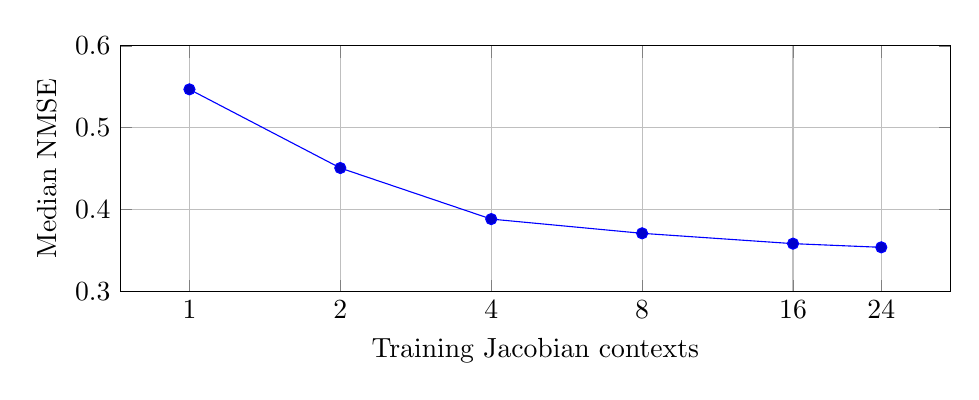
\begin{tikzpicture}
\begin{axis}[
  width=\linewidth,height=4.7cm,
  xmode=log,log basis x=2,
  xtick={1,2,4,8,16,24},xticklabels={1,2,4,8,16,24},
  xlabel={Training Jacobian contexts},ylabel={Median NMSE},
  ymin=0.30,ymax=0.60,grid=major]
\addplot+[mark=*] coordinates {
  (1,0.5468) (2,0.4507) (4,0.3883) (8,0.3709) (16,0.3583) (24,0.3538)};
\end{axis}
\end{tikzpicture}
\end{minipage}\hfill
\begin{minipage}{0.48\linewidth}
\centering
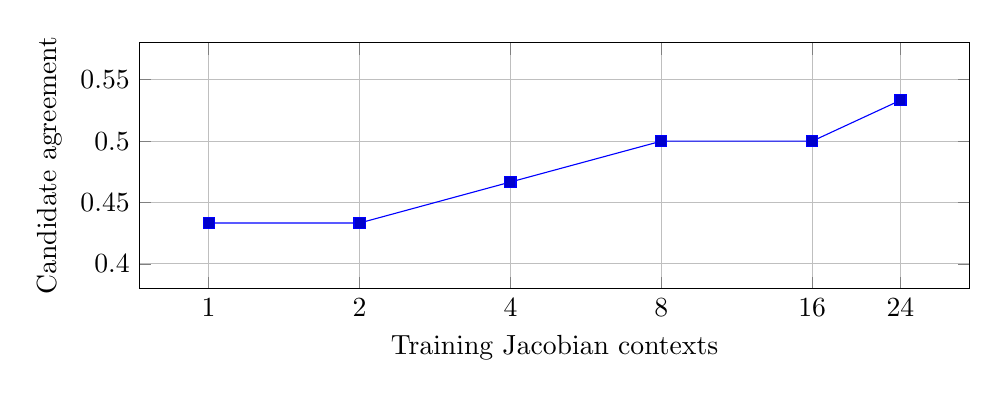
\begin{tikzpicture}
\begin{axis}[
  width=\linewidth,height=4.7cm,
  xmode=log,log basis x=2,
  xtick={1,2,4,8,16,24},xticklabels={1,2,4,8,16,24},
  xlabel={Training Jacobian contexts},ylabel={Candidate agreement},
  ymin=0.38,ymax=0.58,grid=major]
\addplot+[mark=square*] coordinates {
  (1,0.4333) (2,0.4333) (4,0.4667) (8,0.5000) (16,0.5000) (24,0.5333)};
\end{axis}
\end{tikzpicture}
\end{minipage}
\caption{Registered capital-validation averaging curves.  Medians at 1--16
contexts use 128 fixed draws; 24 contexts is the single full training mean.
Evidence level: \level{Specificity} within one relation/model.}
\label{fig:averaging}
\end{figure}

\subsection{Population averaging helps in a bounded relation}

On 30 previously unanalyzed validation outcomes from the capital relation, the
24-training-context population Jacobian improves normalized logit MSE from
$0.737$ for the matched local Jacobian to $0.354$, correlation from $0.835$ to
$0.866$, and candidate agreement from $0.300$ to $0.533$.  It has lower MSE in
exactly four of six recipient contexts.  A paired-bootstrap raw-MSE improvement
interval is $[2.28,8.28]$ with estimated positive probability $0.9997$.
This interval resamples the 30 donor outcomes as if independent; because five
donors share each of only six recipients, it is descriptive outcome-level
uncertainty and not a recipient-clustered confidence interval.

The averaging curve improves median MSE from $0.547$ at one context to $0.354$
at 24 contexts, with fixed log-size/MSE correlation $-0.915$.  Answer-row
permutations have p05 MSE $1.413$ and p95 agreement $0.033$, supporting semantic
specificity.  Nevertheless, quadratic Taylor obtains the best candidate
agreement ($0.833$) despite worse continuous MSE ($0.774$).  Thresholds were
chosen after an exploratory test-split observation and confirmed only on the
previously unused validation entities.  Population averaging is prior art and
the result is neither a method novelty nor a circuit.

More generally, the 612 capital patches are intervention outcomes rather than
612 independent semantic units.  Accuracy is estimated on six held-out
entities per split, and the reported transfer/agreement rates currently lack
entity- or donor-clustered intervals.  The tables therefore retain raw rates
and bounded dispositions rather than population-level significance claims.

\begin{table}[t]
\centering
\small
\caption{Held-out capital validation comparison (30 outcomes).}
\label{tab:population}
\begin{tabular}{@{}lrrrl@{}}
\toprule
Transport & NMSE & Corr. & Candidate agr. & Evidence level \\
\midrule
Exact local JVP & 0.737 & 0.835 & 0.300 & \level{Specificity} \\
Train population JVP & \textbf{0.354} & 0.866 & 0.533 & \level{Specificity} \\
Quadratic Taylor & 0.774 & \textbf{0.910} & \textbf{0.833} & \level{Specificity} \\
\bottomrule
\end{tabular}
\end{table}

\subsection{Registered threshold-and-grid boundary rules do not generalize}

The element, one-shot state, and country-code studies all pass their numerical
audits and exhibit answer-row-aligned late-layer population transport beyond
answer-row nulls.  The earlier zero-shot state study passed numerics but failed
its competence gate and decided no hypothesis.  The stronger
temporal-geometric hypotheses do not survive.
For one-shot states, donor control crosses at layer 24 on validation while
population advantage crosses at layer 26; test aligns at 24, and an early
control gate also fails.  For country codes, validation population advantage
crosses at layer 21 before 50\% donor control crosses at 24; test crosses both
at 21.  This is the opposite of the preregistered direction requiring the
population crossing not to precede causal control.

Country-code direct donor transfer progresses as
$0,.367,.867,1.0$ on validation and $0,.667,.967,1.0$ on test over layers
18/21/24/26.  At test layers 21 and 26, population NMSE/agreement are
$0.2949/0.5667$ and $0.01470/0.9667$, versus row-null p05 MSE
$1.350/1.679$ and p95 agreement $0.233/0.100$.  Answer-row specificity is
strong, but the registered threshold-and-grid ordering rules fail across these
prompt families and splits on Qwen3-0.6B.  This does not exclude a different
continuous boundary or a result on a denser layer grid.

\begin{table*}[t]
\centering
\small
\caption{Preregistered layer-geometry conclusions.  ``Pass'' refers only to
the named hypothesis, not a circuit or workspace.}
\label{tab:layer}
\begin{tabularx}{\textwidth}{@{}p{2.8cm}p{3.0cm}p{2.5cm}p{2.1cm}Y@{}}
\toprule
Relation & Strong claim & Held-out outcome & Evidence level & Interpretation \\
\midrule
Elements & H-LLM-08; H-GEO-08/09; H-CROSS-03 & Pass; fail/pass; fail & \level{Specificity} & Donor control and row specificity pass; strict inversion/conjunction fail. \\
States, zero-shot & H-LLM-10; H-GEO-10/11; H-CROSS-04 & Undecided & \level{Availability} & Clean validation/test accuracy $0.667/0.667$ fails the frozen behavior gate. \\
States, one-shot & H-LLM-12; H-GEO-12/13; H-CROSS-05 & Fail; fail/pass; fail & \level{Specificity} & Validation population onset lags control by one grid step; test aligns. \\
Countries, one-shot & H-LLM-14; H-GEO-14/15; H-CROSS-06 & Pass; fail/pass; fail & \level{Specificity} & Population usefulness precedes 50\% donor takeover on validation; row specificity passes. \\
\bottomrule
\end{tabularx}
\end{table*}

\begin{figure}[t]
\centering
\begin{minipage}{0.48\linewidth}
\centering
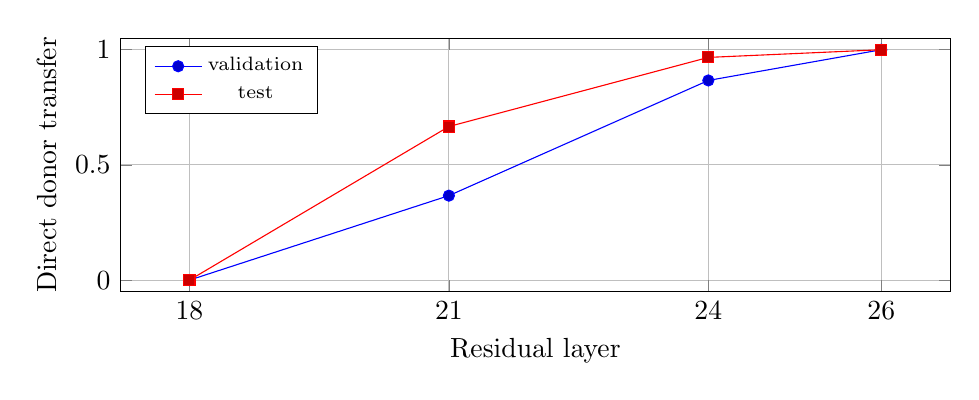
\begin{tikzpicture}
\begin{axis}[
  width=\linewidth,height=4.8cm,
  xtick={18,21,24,26},xlabel={Residual layer},
  ylabel={Direct donor transfer},ymin=-0.05,ymax=1.05,
  legend style={font=\scriptsize,at={(0.03,0.97)},anchor=north west},grid=major]
\addplot+[mark=*] coordinates {(18,0) (21,0.3667) (24,0.8667) (26,1)};
\addlegendentry{validation}
\addplot+[mark=square*] coordinates {(18,0) (21,0.6667) (24,0.9667) (26,1)};
\addlegendentry{test}
\end{axis}
\end{tikzpicture}
\end{minipage}\hfill
\begin{minipage}{0.48\linewidth}
\centering
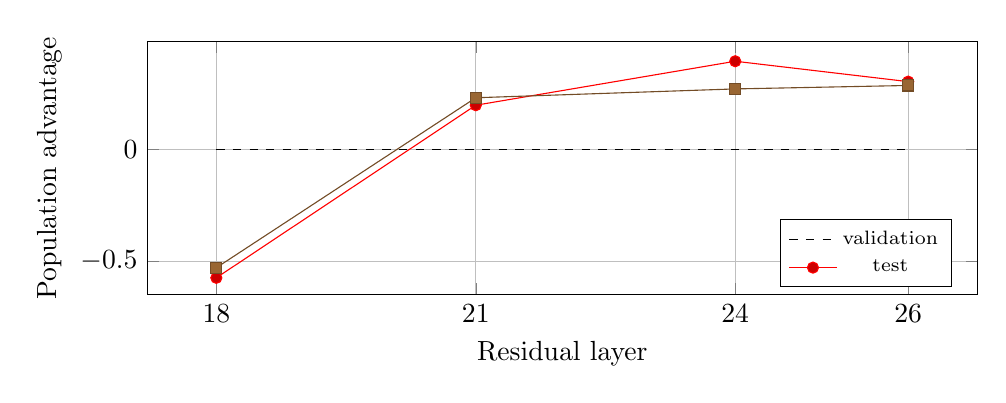
\begin{tikzpicture}
\begin{axis}[
  width=\linewidth,height=4.8cm,
  xtick={18,21,24,26},xlabel={Residual layer},
  ylabel={Population advantage},ymin=-0.65,ymax=0.48,
  legend style={font=\scriptsize,at={(0.97,0.03)},anchor=south east},grid=major]
\addplot+[black,dashed,mark=none] coordinates {(18,0) (26,0)};
\addplot+[mark=*] coordinates {(18,-0.5740) (21,0.1956) (24,0.3917) (26,0.3008)};
\addlegendentry{validation}
\addplot+[mark=square*] coordinates {(18,-0.5290) (21,0.2289) (24,0.2683) (26,0.2837)};
\addlegendentry{test}
\end{axis}
\end{tikzpicture}
\end{minipage}
\caption{Country-code direct control and population advantage over the best
local/quadratic MSE.  Validation population advantage crosses zero at layer 21
before direct donor transfer reaches 0.5 at layer 24; test crosses both at
layer 21.  Evidence level: \level{Specificity}; the registered directional-lag
rule is negative.}
\label{fig:country-layer}
\end{figure}

\subsection{One target-encoder Intervention-JEPA variant fails}

All three target-encoder seeds fail H-LLM-01B, H-LLM-02, and H-LLM-04.  The
predicted meta-latent effective rank is $8.64$--$9.75$, but every EMA target
latent falls below the registered floor of 8 ($6.81$--$7.28$).  That floor may
also reject a useful compact representation and is not decisive by itself.  More
decisively, an oracle decoder given the true target embedding has held-out
normalized MSE $1.065$--$1.753$, showing that failure already exists at the
target-representation/decoder stage rather than only in the predictor.  This
does not distinguish entity dependence, decoder capacity, objective, scale, or
sample size.  Ensemble normalized MSE is $0.930$,
correlation $0.483$, and answer-candidate agreement $0.20$.

Comparator rankings again split by endpoint: exact JVP is best on full-vector
fidelity ($0.599$ normalized MSE), raw linear ridge is best on logit fidelity
($0.329$), and quadratic Taylor is best on direct answer-set behavior ($0.700$
agreement).  PCA-bilinear transport extrapolates catastrophically
($2.04\times10^{11}$ normalized MSE).  These are negative held-out results
for one variant, architecture, dataset split, and prompt family, not a universal impossibility
result for intervention-conditioned JEPAs.

\subsection{Gauge-safe coupling is a control, not a discovered mechanism}

In \code{LLM-CONTEXT-GEOMETRY-001}, reconstruction of stored JVPs from full
Jacobians has median/p95 relative error
$2.86\times10^{-7}/4.58\times10^{-7}$.  Real top-four
pooled/matched/permuted Euclidean overlaps are only
$0.04036/0.03403/0.03286$; registered real-pooling and context-specific
behavior-transport hypotheses fail.  Under a compensated diagonal coordinate
change, naive Euclidean overlap changes by about $120\times$, while the dual
contraction $JD^\top$ is invariant to $1.68\times10^{-16}$.  This verifies a
mathematical identification requirement.  It does not localize a semantic
feature or prove a workspace.

\section{Results: action-conditioned JEPA}

\subsection{Prediction gates pass; circuit and workspace gates do not}

The small LeWorldModel predictive recipe passes its modeling gates in seeds
101, 103, and 107.  Test embedding MSE ranges from $0.134$ to $0.292$,
clean/shuffled-action ratios from $0.155$ to $0.643$, and latent standard
deviation from $0.762$ to $0.862$.  This supports a source-informed small model
reproducing selected design elements; it is not an official checkpoint or
benchmark reproduction.

The broader experiment correctly retains status
\code{FAILED\_REGISTERED\_GATES}.  Hidden patches can recover latent
displacement, but decoded donor-state recovery is negative in two seeds.  The
raw registered restricted-circuit flag passes only seed 107; weak planner
competence and failure of the two-of-three-seed rule prevent treating that flag as a valid
level-5 circuit.  The clean planner succeeds on only one of 12 cases per seed,
so planner changes are not evidence of useful planning.  The proxy workspace
readout candidate passes in zero seeds, and matched random subspaces can damage
the post-hoc consumers more strongly.  We therefore report: no
candidate passed the registered post-hoc workspace-proxy tests in the studied
models and controls.  Because the five consumers are post-hoc readouts rather
than independently used modules, even a positive proxy would not by itself
establish a workspace.  We do not claim that JEPAs in general lack
workspace-like representations.

\begin{table}[t]
\centering
\small
\caption{Small LeWorldModel disposition across three model seeds.}
\label{tab:world}
\begin{tabular}{@{}lcll@{}}
\toprule
Criterion & Passing seeds & Result & Evidence level \\
\midrule
Predictive reproduction & 3/3 & Pass & \level{Availability} \\
Planning-specificity flag & 2/3 & Mixed & \level{Specificity} \\
Hidden latent+decoded mediation & 1/3 & Reject & \level{Causal mediation} \\
Raw restricted-circuit flag & 1/3 & Ineligible/reject & \level{Causal mediation} \\
Competent planner & 0/3 & Ineligible & \level{Availability} \\
Workspace proxy & 0/3 & Null & \level{Availability} \\
\bottomrule
\end{tabular}
\end{table}

\subsection{The first recurrent population study is numerically rejected}

\code{WM-POPULATION-JACOBIAN-001} compares local and population action
Jacobians in decoded physical coordinates and includes a condition-100 latent
reparameterization control.  Its status is
\code{REJECTED\_NUMERICAL\_GATE}: the original 12-node path integral is
underresolved for sharply cancelling recurrent chords.  A no-write diagnostic
reduces the worst seed-103 relative integration error from $49.8$ at 12 nodes
to $0.0058$ at 192 nodes.  Because the registered numerical gate failed, none
of its favorable method rankings is scientific evidence.  In particular, the
within-context vertex-mean MSE result is also confounded by scalar shrinkage
and is not promoted.

\subsection{Action-path cancellation remains calibration only}

The first validation-only action-path calibration profiles 24 chords per seed
and horizon.  Horizon-one maximum direct-reconstruction/refinement errors are
below $0.00077/0.00169$ across seeds.  Horizon four converges at the original
resolution for seed 107 ($0.00197/0.00093$) but not seeds 101
($0.0680/0.1369$) or 103 ($0.478/2.059$).

At 512/1024 nodes, V2 reduces horizon-four maximum
integration/refinement errors to $0.01291/0.02605$, $0.03394/0.03141$, and
$0.001393/0.000250$ for seeds 101, 103, and 107.  The first two seeds therefore
remain underresolved.  Median horizon-four cancellation ratios are $2.589$,
$5.261$, and $1.174$ for
seeds 101, 103, and 107, while local relative-error medians are $2.023$,
$1.389$, and $0.972$.  Cancellation/error Spearman correlations are
$0.415/0.478/0.857$, exceeding within-action-pair null p95 by only
$0.0454/0.0283/0.0165$.  Horizon-four versus horizon-one cancellation
amplification is $1.05/2.82/0.983$, so recurrence amplification is not
replicated.  Table~\ref{tab:path} retains these measurements as availability
and numerical-calibration evidence only.

Moreover, cancellation $\kappa=L/\lVert\Delta y\rVert$ and normalized local
error share the denominator $\lVert\Delta y\rVert$.  Their raw correlation can
therefore increase mechanically for small net effects.  Action-pair
stratification does not remove this confound.  Any confirmatory continuation
must preregister unnormalized or partial-association endpoints and permutations
conditioned on direct-effect magnitude; quadrature convergence alone is not
sufficient.

Before the V2 artifact existed, adversarial design review rejected a proposed
derived denominator audit before commit.  V2 checks convergence of an
integrated vector, but does not store scalar path length at both resolutions;
the recorded direct norm is clamped, and only two chords are available per
action pair.  Consequently, separate action-pair and effect-size-bin
permutations cannot establish a joint conditional null.  We retain V2 only as
numerical/vector calibration and close this route in the small model without
accessing protected test goals.  Reopening requires a new prospective data
collection with raw norms, scalar path-length refinement, substantially denser
within-pair sampling, row-level split guards, and a preregistered joint null.

\begin{table*}[t]
\centering
\small
\setlength{\tabcolsep}{3pt}
\caption{Decoded recurrent action-path calibration.  V2 uses the identical
validation chords with streamed exact Jacobians at 512/1024 nodes.}
\label{tab:path}
\begin{tabular}{@{}p{0.8cm}p{0.8cm}p{1.55cm}p{1.55cm}p{1.45cm}p{1.55cm}p{1.75cm}p{1.7cm}@{}}
\toprule
Seed & $h$ & Median $\kappa$ & Median local error & Spearman & Null p95 & \shortstack{Max integ./\\refine error} & Evidence level \\
\midrule
101 & 4 & 2.589 & 2.023 & 0.415 & 0.369 & \shortstack{0.0129/\\0.0261} & \level{Availability} \\
103 & 4 & 5.261 & 1.389 & 0.478 & 0.450 & \shortstack{0.0339/\\0.0314} & \level{Availability} \\
107 & 4 & 1.174 & 0.972 & 0.857 & 0.841 & {\scriptsize\shortstack{0.00139/\\0.000250}} & \level{Availability} \\
\bottomrule
\end{tabular}
\end{table*}

The retained interpretation is narrower than a geometry claim.  Some acquired
model/context pairs have large decoded derivative arc length relative to their
net effect, but two seeds remain underresolved and the shared denominator can
mechanically couple cancellation to local error.  The artifact therefore does
not show that a single local vector is causally insufficient.  Protected test
goals were not touched.

\section{Cross-track synthesis}

Three conclusions survive the combined audit.

First, \emph{finite intervention transport is endpoint-dependent}.  In Qwen,
exact local transport can dominate vector MSE while a quadratic or population
transport better predicts answer behavior.  A surrogate's aggregate effect
correlation is therefore insufficient for mechanistic ranking.

Second, \emph{the registered threshold-and-grid boundary rules do not
generalize}.  Answer-row-aligned population Jacobians become highly predictive
in late Qwen layers, but the first useful grid point can precede, coincide with,
or follow a fixed donor-control threshold across relations and splits.  This
falsifies the named rules on the studied four-layer grids, not every possible
continuous boundary.

Third, \emph{learned compression and shared sensitivity are not mechanism
proofs}.  The tested target-encoder Intervention-JEPA can produce a nontrivial predicted
latent rank while its target geometry and oracle decoding fail to generalize.
Likewise, a small JEPA bottleneck and several sensitive heads do not establish
a workspace when matched controls and planner competence fail.

The tempting stronger synthesis---that Qwen and action-conditioned JEPAs share
one causal workspace geometry---is unsupported.  Qwen's current positive
result concerns population transport of factual-answer logits; the JEPA
candidate concerns decoded recurrent action paths.  Sharing an intervention
schema does not establish shared semantics or shared mechanism.

\section{Limitations}

\begin{itemize}[leftmargin=*]
  \item The main causal LLM evidence uses Qwen3-0.6B.  Qwen3-4B has only a
  bounded activation-capture smoke test; no cross-scale mechanism is claimed.
  \item Factual studies use narrow templates and only six entities in each
  held-out validation/test split.  The population confirmation contains 30
  held-out donor outcomes but only six recipient clusters, and its interval is
  not recipient-clustered.
  \item Population averaging and late crystallization are prior art.  Our
  contribution is the bounded direct comparison and the failed stronger
  hypotheses, not a new estimator.
  \item We have not localized a robust head/MLP circuit, reconstructed a Qwen
  circuit, or shown cross-task mode reuse.
  \item The capital donor-patch dataset establishes mediation but lacks matched
  subspace/covariance corruptions and incompatible-donor controls for
  specificity.  Its aggregate top-token-change and approximation metrics are
  train-weighted.
  \item The target-encoder Intervention-JEPA is evaluated on one factual patch
  family.  Its negative result may reflect entity-dependent target geometry,
  limited data, architecture, or objective.
  \item The binding-mediation v1 token audit is an engineering result only and
  its parent design is superseded.  V2 fixes the pre-outcome confounds, but its
  evaluator and protected Qwen execution are not yet complete; it contributes
  no mediator, circuit, JEPA, or workspace evidence in this manuscript.
  \item The LeWorldModel is a source-informed small synthetic model using
  selected design elements.  Its weak planner
  makes behavior-level planning interpretation ineligible.
  \item The official EB-JEPA source contract is pinned and its recurrent sites
  are implemented, but no trained checkpoint or local planning result is yet
  reported.  The upstream Python 3.12/PyTorch 2.6 pin is CPU-only on this SM120
  host; local GPU execution requires a disclosed Torch 2.10/cu128 deviation.
  Consequently a later model run can reproduce source/config semantics but not
  claim bitwise dependency equivalence.
  The Two Rooms dependency declaration omits three imported packages, and an
  exploratory MPPI action exceeded its configured norm.  Integration V1 is
  superseded for incomplete RNG control; corrected integration passes exact
  replay, and the planner bound defect is confirmed.  Neither establishes
  trained planning competence.
  \item The first JEPA population-transport study is numerically rejected.  The
  action-path study remains validation-only calibration.  Its cancellation/error
  association has a shared-denominator confound, and the parent artifact omits
  the diagnostics and sampling support needed for a retrospective repair; that
  route is closed without protected-test access.
  \item No positive circuit reaches evidence level 5, and no result reaches a
  broad multi-model level-6 mechanism claim.
\end{itemize}

\section{Reproducibility}

All configurations, source, compact metrics, provenance records, and tests are
versioned.  Large weights, raw activation shards, and caches are excluded from
Git.  Qwen uses revision
\texttt{\seqsplit{c1899de289a04d12100db370d81485cdf75e47ca}} with FP32/eager attention,
TF32 and autocast disabled for derivative studies.  Capital patches edit
\code{blocks.21.resid\_post} and measure \code{blocks.27.resid\_post} plus 36
answer logits; the older audit grid additionally uses source layers 7 and 14.
The small LeWorldModel is source-pinned to official revision
\texttt{\seqsplit{8edfeb336732b5f3ce7b8b210d0ba370a09e2cac}}; the EB-JEPA contract target is
pinned to \texttt{\seqsplit{966e61e9285b3a876f49b9774e9720d9a99a7925}}.  The reported RTX host uses
Python 3.14.2, PyTorch 2.10.0+cu128, Transformers 5.3.0, NVIDIA driver 591.86,
and a 12,227 MiB RTX 5070 Ti Laptop GPU.  Every prompt, entity roster, split,
donor rule, seed, dtype, site, and threshold is stored in the named YAML
configuration and hypothesis registration.  The principal artifacts are:

\begin{itemize}[leftmargin=*]
  \item \code{artifacts/metrics/qwen\_jvp\_audit\_v2.json} (run commit
  \code{a779ff6});
  \item \code{artifacts/metrics/qwen\_capital\_patch\_dataset\_v1.json}
  (\code{95018cb});
  \item \code{artifacts/metrics/qwen\_target\_ijepa\_v1.json}
  (\code{3086cd4});
  \item \code{artifacts/metrics/qwen\_population\_jacobian\_v1.json}
  (\code{3725714});
  \item \code{artifacts/metrics/qwen\_country\_code\_layer\_geometry\_v1.json}
  (\code{48226c6});
  \item \code{artifacts/metrics/lewm\_small\_reproduction\_v1.json}
  (\code{4dbc388});
  \item \code{artifacts/metrics/lewm\_action\_path\_calibration\_v1.json}
  (\code{eb943a5});
  \item \code{artifacts/metrics/eb\_jepa\_contract\_smoke.json}
  (\code{979c2d6});
  \item \code{artifacts/metrics/lewm\_action\_path\_calibration\_v2.json}
  (clean \code{288f663}; 19,176.20 seconds).
  \item \code{artifacts/metrics/eb\_jepa\_runtime\_compatibility.json}
  (clean \code{15d88ce}; all eight frozen gates pass).
  \item \code{artifacts/metrics/eb\_jepa\_two\_rooms\_integration\_v2.json}
  (clean \code{9a18008}; exact two-process fingerprint replay).
  \item \code{artifacts/metrics/eb\_jepa\_planner\_constraint.json}
  (clean \code{da30443}; all seven post-discovery gates pass).
\end{itemize}

Each experiment is replayed with
\code{python scripts/run\_experiment.py --config <config>}; dataset creation
uses the correspondingly registered generator.  Ignored HDF5 shards are
regenerated from pinned model revisions/configs and verified against committed
sizes and SHA-256 checksums.  The repository remote is
\url{https://github.com/Kripta-Studios/causal-workspace-jepa}; access to any
non-public revision must be obtained from the maintainers.  No private user
conversation, secret, or credential is research data.

The repository-level audit checks metric/provenance pairs, tracked checksums,
preregistered IDs, documentation consistency, and clean-commit execution.
Unit, integration, and scientific tests are run together with Ruff and Python
bytecode compilation.  Exact continuation commands and hardware profiles are
recorded in \code{VPS\_RUNBOOK.md} and \code{docs/REPRODUCIBILITY.md}.

\subsection*{Code and data availability}

Source, registrations, compact metrics, provenance, manifests, tests, and this
manuscript are versioned in the repository above.  Public model weights remain
at their upstream Hugging Face or official-code sources.  Generated raw data,
weights, activation shards, and LaTeX products are intentionally untracked;
their reconstruction commands and integrity metadata are committed.  The
paper should be cited only together with the exact repository commit used to
produce a reported table.

\section{Conclusion}

The strongest result of this work is not a newly discovered workspace.  It is
a corrected empirical boundary on what the current evidence can support.
Exact FP32 local and quadratic transports overturn an apparent learned
Intervention-JEPA advantage; direct capital patches establish a real causal
behavior dataset; population Jacobians improve some finite effects but do not
obey the registered control--predictivity rules across the studied factual
families and four-layer grids; and one target-encoder JEPA variant fails its
registered held-out gates.  In the physical track, predictive gates pass while
circuit and workspace acceptance gates fail.  Decoded recurrent action-path
cancellation is closed as a scientific route in the current small model because
the acquired artifact cannot identify the proposed geometry.  The official
EB-JEPA one-layer recurrence is now exactly decomposed and intervention-ready,
but remains random-weight engineering evidence.  Its official MPPI planner also
ignores a configured action-norm bound that CEM enforces; the environment supplies
no fallback check.  The next discriminating studies should use a precisely
replayed, episode-paired Qwen treatment to compare frozen module mediator rankings and reproduce the
competent official EB-JEPA planner under both original and corrected MPPI before
auditing recurrent action routes.  Only an eligible causal dataset from
the former can support a new trajectory Intervention-JEPA test.  Direct held-out
behavior, grouped uncertainty, cross-model replication, and controls separating
native mechanism from flexible prediction remain mandatory.

\bibliographystyle{plain}
\bibliography{references}

\end{document}
